\subsection{Applikationen (Jens)}
 
\begin{figure}[H]
    \centering
   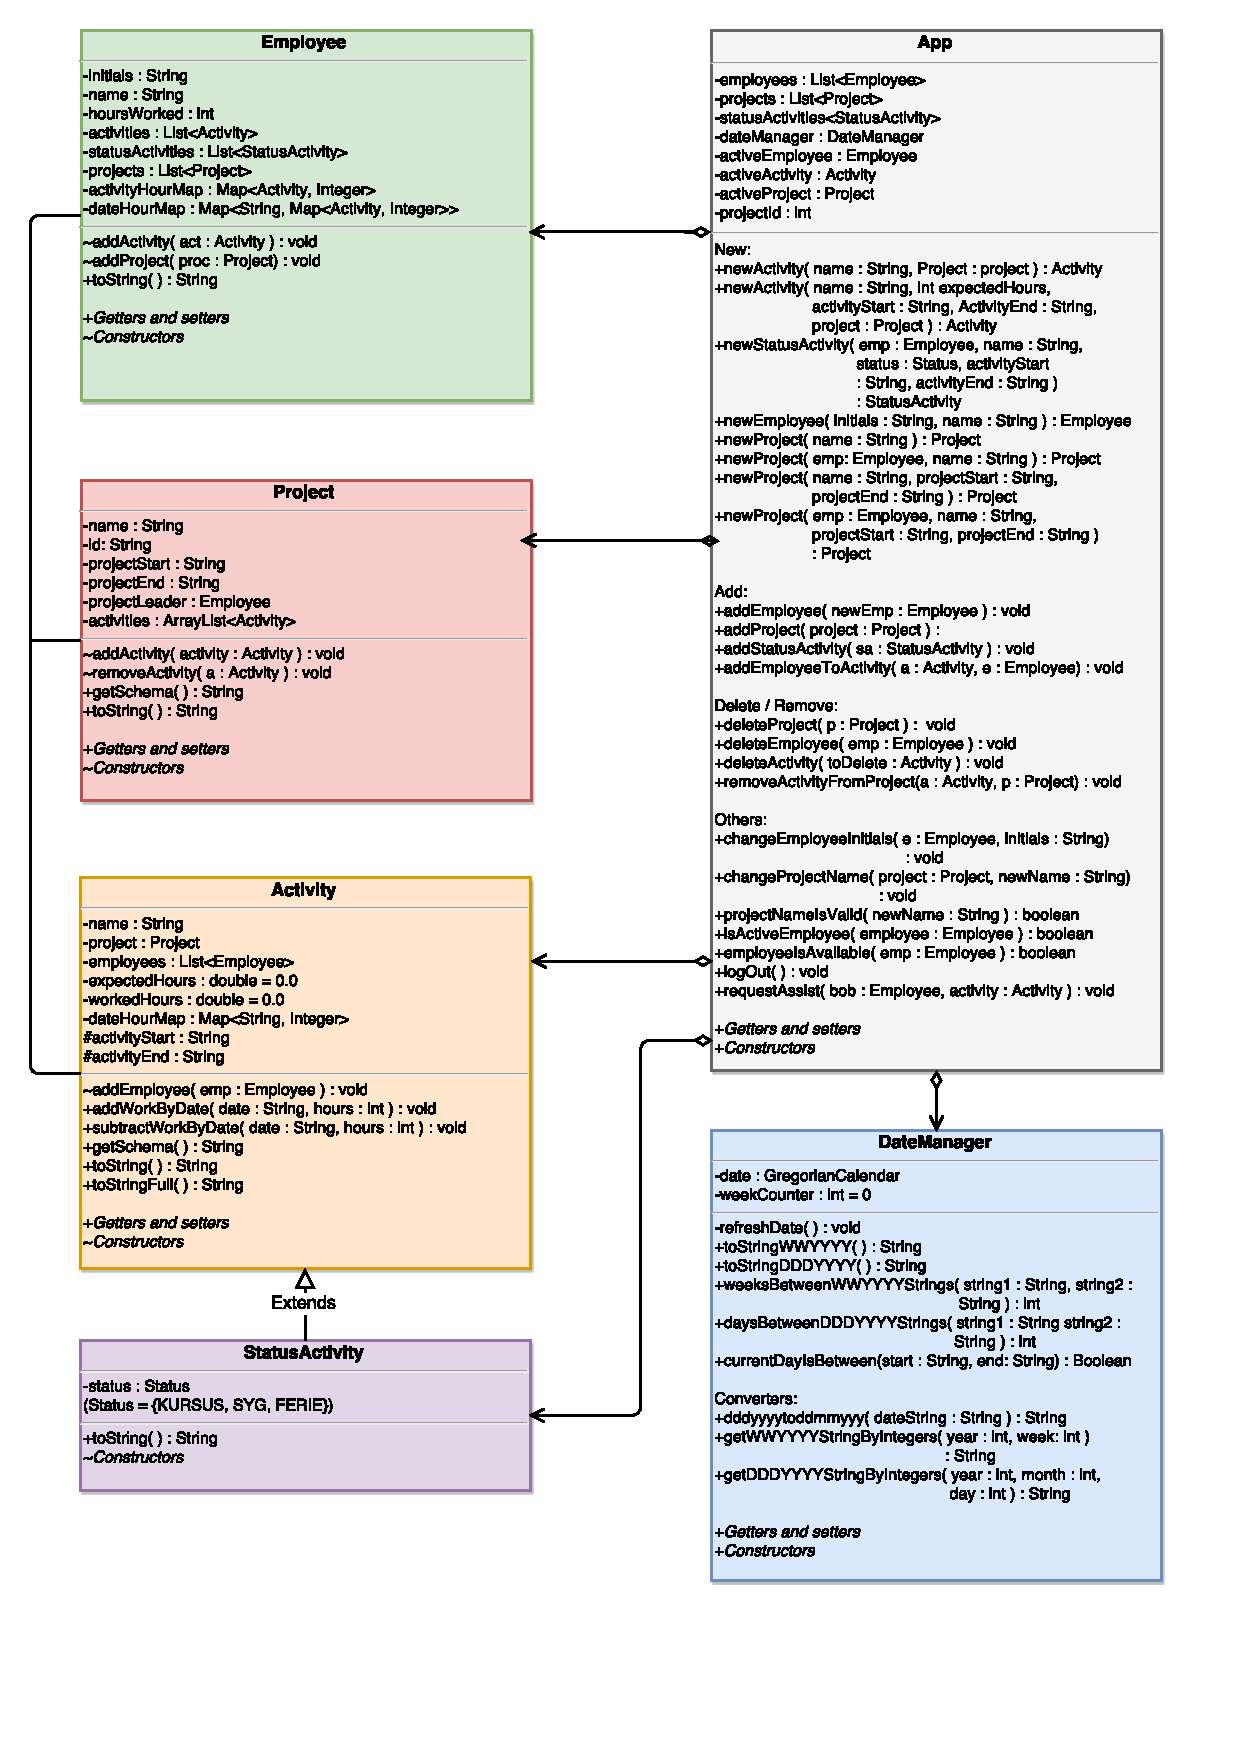
\includegraphics[width = \textwidth]{Figurer/SE2UML.pdf}
    \caption{Klassediagram over applikationen under brugerinterfacet. Diagrammet viser hvordan \texttt{App} har den overordnede kontrol, samt instanser af de andre klasser. For at sikre at de forskellige klasser bliver tilgået korrekt, er filerne placeret i sin egen \texttt{app.src} pakke, og mange metoder samt fields har private eller pakke scope. 
    }
    \label{fig:SE2UML}
\end{figure}
%% Roar start
%Under bruger interfacet er applikationen bygget op af klasserne set på %figur \ref{fig:SE2UML}. Diagrammet viser hvordan \texttt{App} har den %overordnede kontrol, samt instanser af de andre klasser. Klassen %\texttt{App} er sat op som porten mellem brugeren og applikationen selv, %og indeholder information om hele systemet, hvormod fx \texttt{Employee} %klassen ikke har informationer om de andre medarbejdere eller projekter de %ikke er del af. For at sikre at de forskellige klasser bliver tilgået %korrekt, er filerne placeret i sin egen \texttt{app.src} pakke, og mange %metoder samt fields har private eller pakke scope. Dermed kontrolleres %at fx tilføjelse af nye medarbejdere sker gennem metoden i \texttt{App}, %og ikke \texttt{Employee}'s konstruktør direkte.
%% Roar slut
Som nævnt i forrige afsnit er programmet bygget op efter Model-View-Controller designmønsteret. Dette afsnit omhandler 'Model' delen. Alle klasser, der er nødvendige for at modellere et projektplanlægningsprogram, ligger i pakken \texttt{app}. Foruden \texttt{exception}-filer kan hele modellen ses i UML-diagrammet på figur \ref{fig:SE2UML}. Dette afsnit beskriver overordnet hvordan modellen er struktureret (afsnit \ref{totrin}) efterfulgt af nogle bemærkelsesværdige pointer omkring dette (afsnit \ref{totrin}, \ref{activefelter} og \ref{datomanager}). Til sidst gennemgås vigtige ændringer siden rapport 1 (afsnit \ref{aendringer}).

\subsubsection{To-trins pyramiden}
\label{totrin}
Kontrol-flowet i modellen er hierarkisk bygget op som en to-trins pyramide (se figur \ref{fig:totrin}). \texttt{App.java} sidder på toppen og er den primære interaktionskilde for programmets Controllere (der ligger i \texttt{gui} pakken). Her bliver alle instanser af medarbejdere, projekter og aktiviteter\footnote{\textbf{En lille undtagelse} til den beskrevne hierarkiske struktur, er hvordan \texttt{App} tilgår allerede eksisterende aktiviteter. Disse bliver nemlig ikke gemt i en liste under \texttt{App}, men kan findes under hvert projekts \texttt{activities} liste. Da hvert \texttt{Activity} objekt har et felt med dens tilknyttet \texttt{Project}, kunne en samlet liste over aktiviteter godt laves i \texttt{App} uden at miste information. Denne struktur er dog ikke brugbar for programmets formål og blev derfor fravalgt, også for at spare plads.} samlet, tilgået og administreret. Nye \texttt{Project}, \texttt{Activity} og \texttt{Employee} objekter bliver konstrueret og destrueret (indirekte\footnote{Destruktion foregår direkte ved Java's garbage collection.}) gennem metoder i \texttt{App} og brugte objekter bliver gemt, og holdt styr på, i lister. 
\begin{figure}[H]
    \centering
    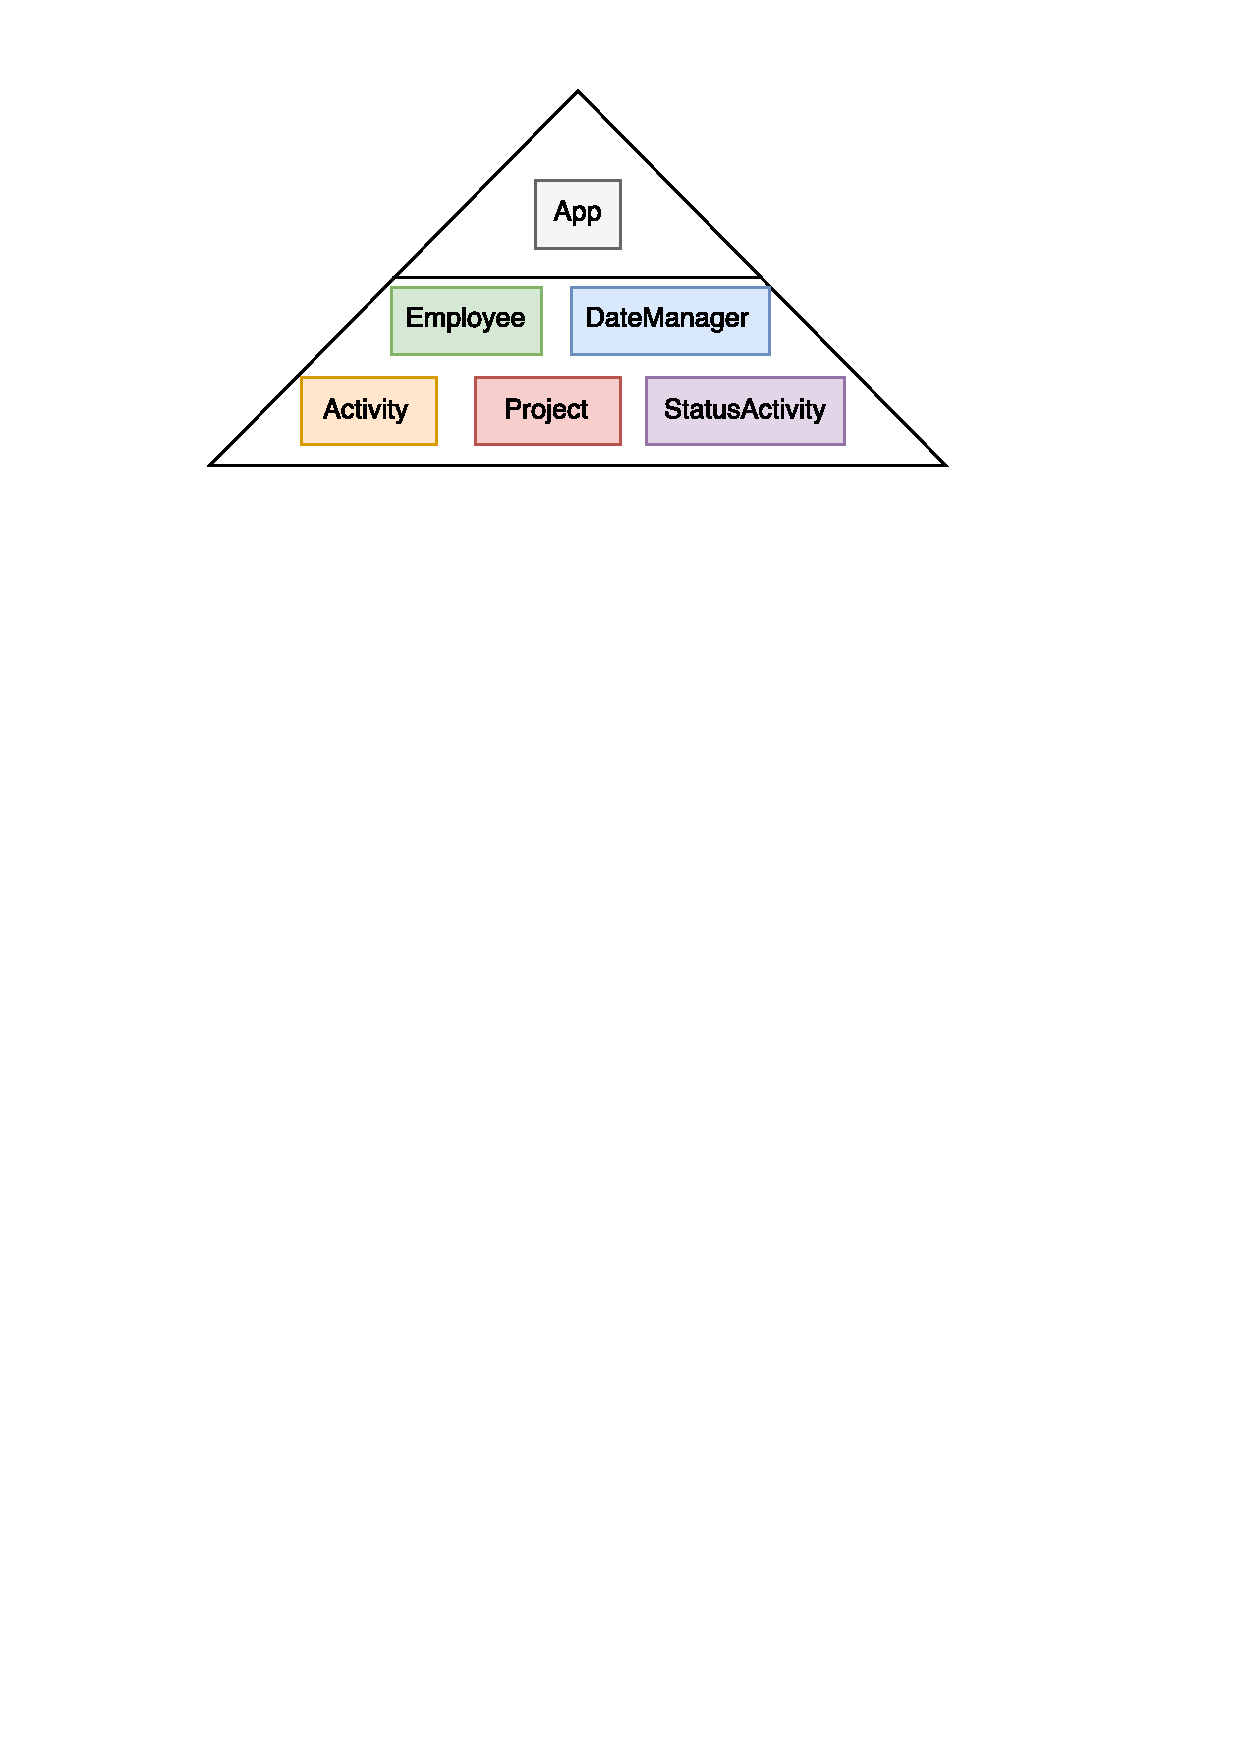
\includegraphics[scale = 0.8]{Figurer/totrin.pdf}
    \caption{Illustrering af kontrol-flowet i modellen. Pyramiden repræsentere det hierarkisk to-delte forhold mellem klasserne i modellen, og hver firkant repræsenterer en klasse. \texttt{App} holder styr på resten af modellens dataklasser som findes I bunden af pyramiden.}
    \label{fig:totrin}
\end{figure}
I bunden af pyramiden findes resten af klasserne; \texttt{Employee}, \texttt{Project}, \texttt{Activity}, \texttt{StatusActivity} og \texttt{DateManager}. Disse fungerer alle sammen som augmenterede data-klasser med metoder hvorigennem modifikation og tilgang af data kan ske. Desuden indeholder de diverse belejlige metoder til formattering af data (som fx \texttt{toString()} og \texttt{getSchema()}, der returnerer en streng med specifik information om instansen). 


\subsubsection{\texttt{Employee}-\texttt{Project}-\texttt{Activity} treenigheden}
\label{Figurer/treenighed.pdf}
Som det også kan bemærkes på UML-diagrammet (figur \ref{fig:SE2UML}) er klasserne \texttt{Employee}, \texttt{Project} og \texttt{Activity} stærkt sammenflettet:
\begin{itemize}
    \item \texttt{Employee} har en liste af typen \texttt{List<Activity>} (\texttt{activities}) og en af typen \texttt{List<Project>} (\texttt{projects}).
    \item \texttt{Project} har et felt af typen \texttt{Employee} (\texttt{projectLeader}) og en liste af typen \texttt{ArrayList<Activity>} (\texttt{activities}).
    \item \texttt{Activtiy} har et felt af typen \texttt{Project} (\texttt{project}) og en liste af typen \texttt{List<Employee>} (\texttt{employees}).
\end{itemize}
Treenigheden er stærkt afhængig af hinanden, men er fuldkommen upåvirket af alt andet. På den måde kan de i fællesskab ses som en atomar kerne i modellen for projektplanlægnings programmet. 
%\textit{Deres fælles afhængighed gør dem ude %af stand til at eksistere uden hinanden. På %trods af dette er blablalbalbla skriv noget om %at det er den atomare kerne af modellen og at %suppe herakien gør det let og intuitivt at %navigere rundt i}
\begin{figure}[H]
    \centering
    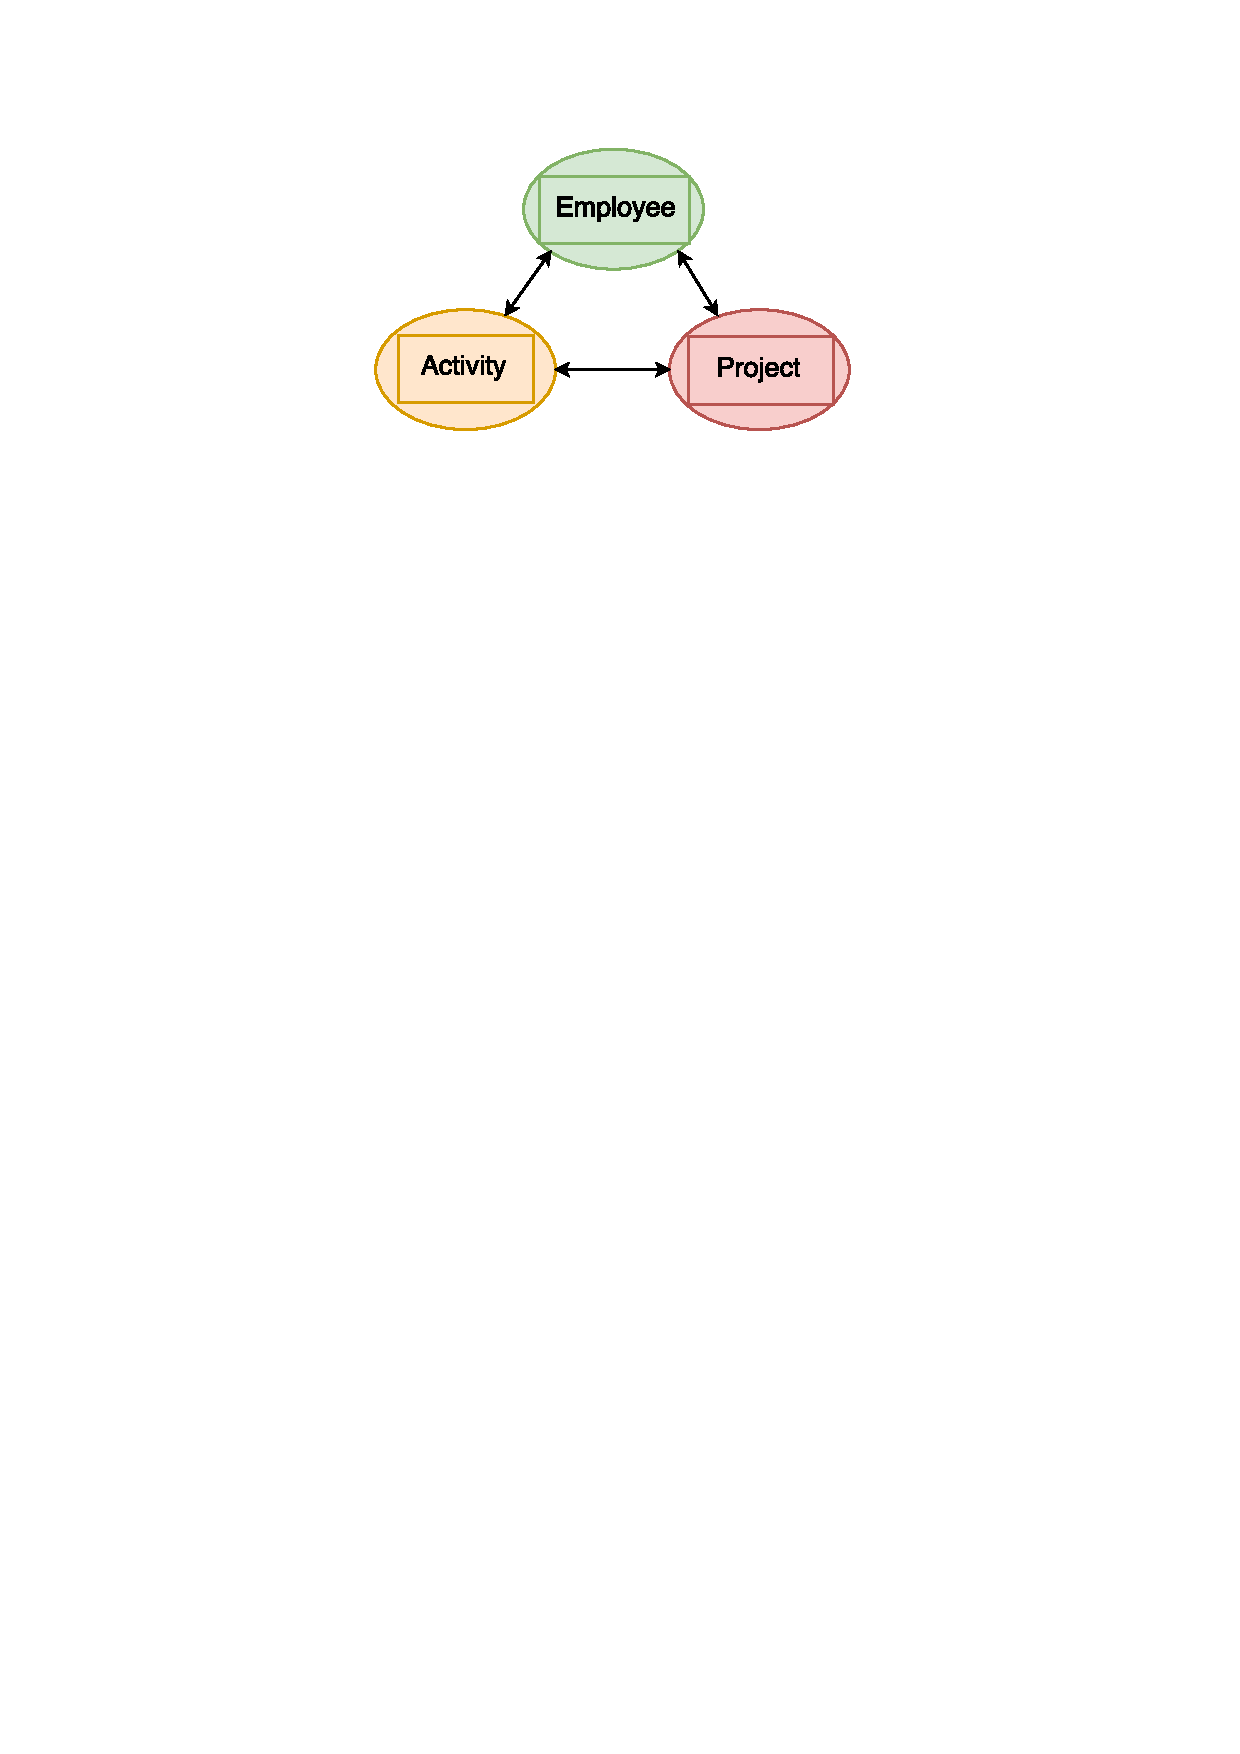
\includegraphics[scale = 0.8]{Figurer/treenighed}
    \caption{Den sammenkoblede natur gør modellen relativt ufleksibel, men også intuitiv at bruge. Det er nemt at jonglere mellem instanser af de tre klasser for at finde frem til præcis den information man leder efter. }
    \label{fig:treenighed}
\end{figure}

\subsubsection{\texttt{active} felterne}
\label{activefelter}
I UML-diagrammet på figur \ref{fig:SE2UML} under \texttt{App}-klassen kan tre felter, der hver især starter med 'active', ses: \texttt{activeEmployee}, \texttt{activeActivity} og \texttt{activeProject}. Disse felter bliver sat og læst af Controllere som bruger dem til at afgøre hvad der skal vises på GUI'en.
Fx, hvis der skal vises information om en aktivitet på skærmen, så bliver aktiviteten gemt i \texttt{activeActivity} brugt. Ud fra denne tankegang kan disse felter ses som et lævn fra Controllerene og ikke som en del af modellen (på trods af deres placering). Dog siden vi bruger flere Controllere virker \texttt{App}-klassen som et godt knudepunkt da det i forvejen er Controllerenes fælles reference til modellen og data der skal manipuleres.
%\textit{skriv om at disse felter er et lævn %fra Controlleren og at de måske er lidt %malplaceret i appen, men vi har gjort det så %der er multi-access til activeetellerandet fra %alle de forskellige controllere} 

\subsubsection{Datomanageren}
\label{datomanager}
I implementationen efter rapport 1 viste tidsformattering at være et større problem end forventet. Programspecifikationen krævede ugeopløsning for aktiviteter og projekter, men dagsopløsning til timeregistrering. \texttt{GregorianCalendar}-klassen indeholdt for meget overflødig information til disse to specifikke krav, så vi konstruerede en simpel klasse kaldet \texttt{DateManager}. Klassen indeholder en instans af \texttt{GregorianCalendar} og metoder der konverterer datoer i \texttt{GregorianCalendar} til enten "DDD/YYYY", "WW/YYYY" eller "DD/MM/YYYY" format. Der er også metoder til at sammenligne forskellige datoer i dette forsimplede format. 
%\textit{skriv hva faen den gør og hvorfor vi %har lavet den.}

%% JEG LAVEDE DATEMANAGER, OG DEN BASICALLY BARE SAMMENLIGNER DATOER OG KONVERTERER DATOER TIL DE RIGTIGE FORMATER 

\subsubsection{Ændringer I design siden rapport 1}

Siden sidste iteration af programmet er der sket lidt med hensyn til modellen, som set på figur \ref{fig:SE1UML}. Klasserne \texttt{Projektleder} og \texttt{ProjektAktivitet} er blevet kasseret da deres formål bliver opfyldt af felterne \texttt{projectLeader} og \texttt{activities} i \texttt{Project}. Desuden er hele \texttt{App} og \texttt{DateManager} blevet tilføjet.

\label{aendringer}
\begin{figure}[H]
    \centering
    \includegraphics[width = \textwidth]{Figurer/SE1UML}
    \caption{Klassediagram over programmet fra rapport 1. Kun væsentlige variable er fremhævet.}
    \label{fig:SE1UML}
\end{figure} 


%\textit{skriv om at hele app klassen ikke var der dengagn og %dateserveren blev vi nød til at implementere. Projektaktivitet og %projektleder klasserne er væk siden de viste sig at være overflødige. %Treenigheden er der stadigvæk siden det er kernen i modellen.}

%% OI HER ER DER EN KOMMENTAR DU IKKE HAR SKREVET :) App er basically bare controlleren tbh